\documentclass{article}
\usepackage{tikz}
\usetikzlibrary{arrows.meta}

\begin{document}
\pagestyle{empty}

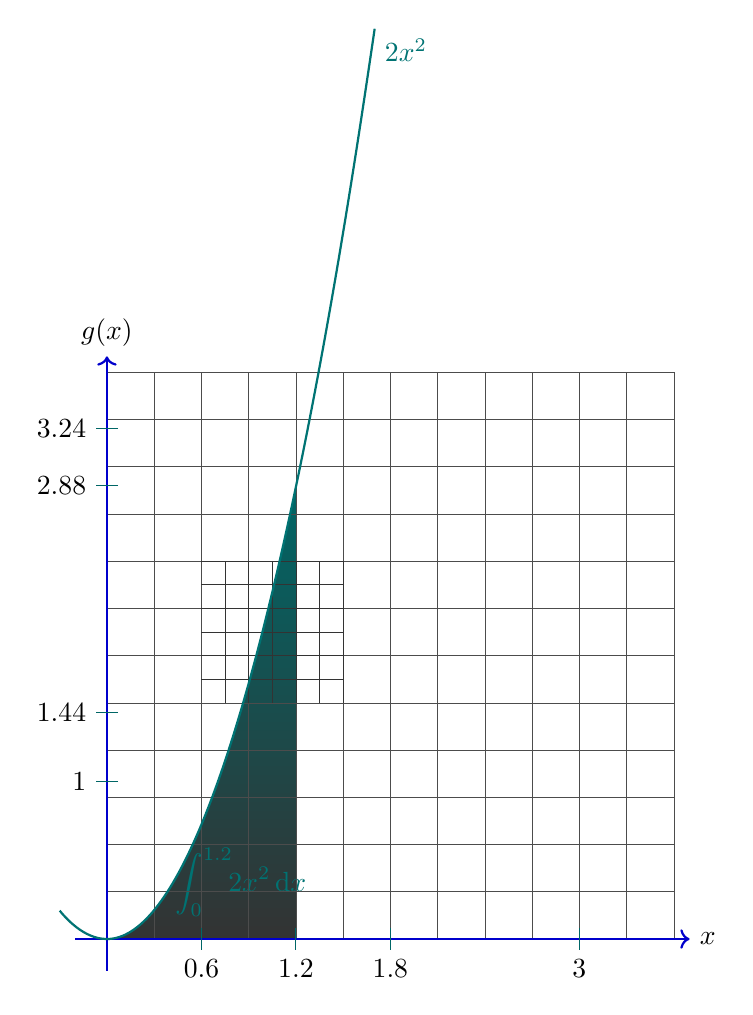
\begin{tikzpicture}[scale=2]
  % Parabola area fill (new colors)
  \shade[top color=teal!80!black, bottom color=gray!40!black] 
      (0,0) parabola (1.2,2.88) |- (0,0);
  % Integral label (updated equation and position)
  \draw (0.85cm,2.3pt) node[above, text=teal!90!black] 
      {$\displaystyle\int_0^{1.2} \!\!2x^2\,\mathrm{d}x$};

  % Grid (modified step and colors)
  \draw[help lines, color=gray!60!black] (0,0) grid[xstep=0.3,ystep=0.3] (3.6,3.6);
  \draw[help lines, color=gray!40!black] (0.6,1.5) grid[xstep=0.15,ystep=0.15] +(0.9,0.9);

  % Axes with new style
  \draw[->, thick, color=blue!80!black] (-0.2,0) -- (3.7,0) node[right, black] {$x$};
  \draw[->, thick, color=blue!80!black] (0,-0.2) -- (0,3.7) node[above, black] {$g(x)$};

  % x-ticks and labels (changed values)
  \foreach \x/\xtext in {0.6/0.6, 1.2/1.2, 1.8/1.8, 3/3}
    \draw[shift={(\x,0)}, color=teal!80!black] (0pt,2pt) -- (0pt,-2pt) node[below, black] {$\xtext$};

  % y-ticks and labels (changed values)
  \foreach \y/\ytext in {1/1, 1.44/1.44, 2.88/2.88, 3.24/3.24}
    \draw[shift={(0,\y)}, color=teal!80!black] (2pt,0pt) -- (-2pt,0pt) node[left, black] {$\ytext$};

  % Parabola (new function: y = 2x^2)
  \draw[thick, color=teal!90!black] (-0.3,0.18) parabola bend (0,0) (1.7,5.78) node[below right, text=teal!90!black] {$2x^2$};
\end{tikzpicture}

\end{document}